\newpage
\section{Theoretical Analysis}
The circuit incorporates three main elements, which are a transformer, an envelope detector, and a voltage regulator.

\subsection{Envelope Detector}
The transformer converts the initial voltage, 230V, to 13.0855V, this last value was taken from ngspice simulation.
The envelop detector incorporates one capacitor and a bridge rectifier.
The function of the bridge rectifier, which consist of four diodes, is to convert the alternating current (AC) input
 that comes from the transformer into a positive current output, with double the frequence. To achieve this it is only necessary to get the absolute value of Vs

\begin{equation}
abs(Vs) = abs(13.0855cos(wt))
\end{equation}
The purpose of the capacitor is to slow the change and flatten the curve.

Knowing that when t $<$ t\textsubscript{OFF}
\begin{equation}
t_{OFF} = \frac{1}{w}atan(\frac{1}{wRC});
\end{equation}

the voltage of the envelope is the absolute value of Vs and when t $>$ t\textsubscript{OFF} the envelope voltage is given by

\begin{equation}
v = 13.0855cos(wt_{OFF})exp(-\frac{t-t_{OFF}}{RC});
\end{equation}
we are able to compute the envelope voltage.


\vspace{-4mm}
\begin{figure}[h] 
    \centering
    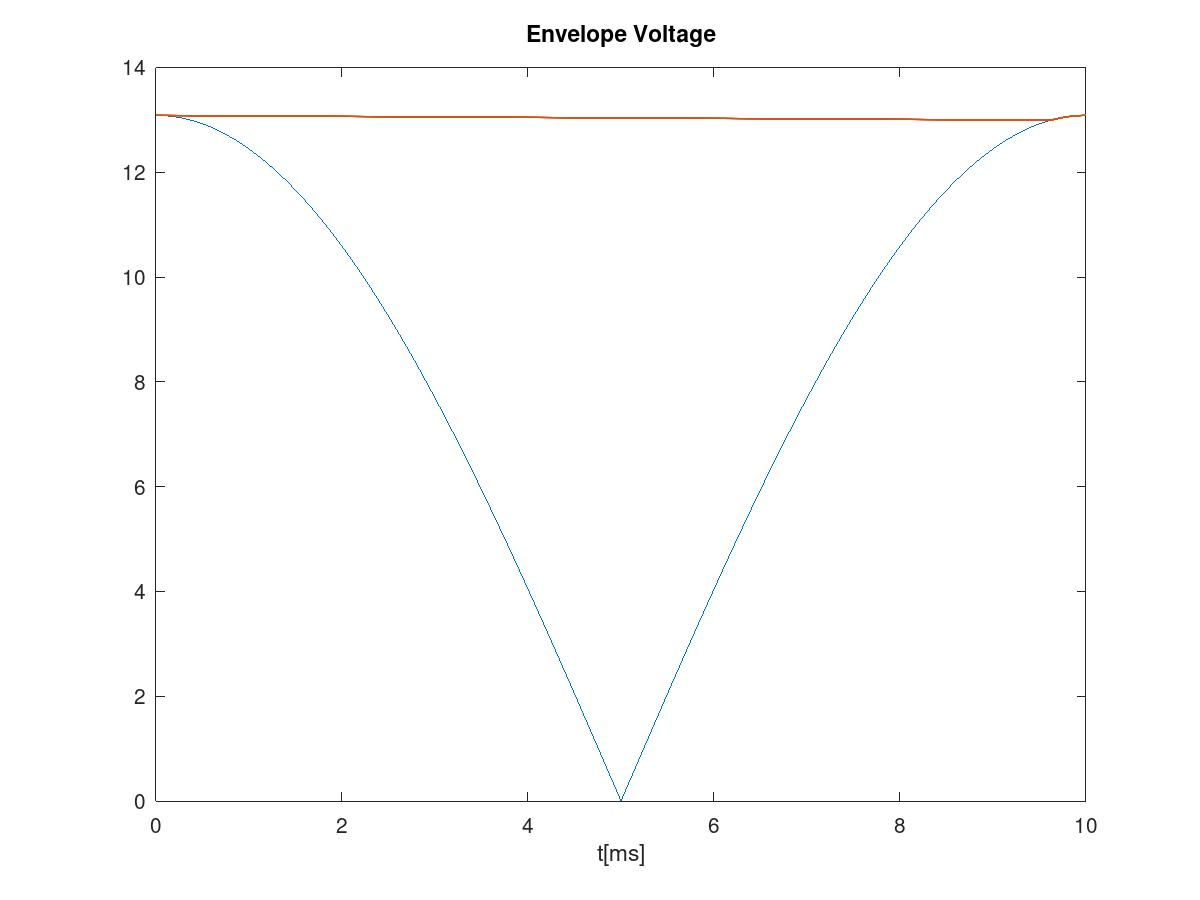
\includegraphics[width=0.75\linewidth]{../mat/venvelope.jpg}
    \caption{Evolution of the voltage at the ends of the capacitor in one half period}
    \label{fig:Envelope Detector}
\end{figure}

\subsection{Voltage Regulator}
In order to minimize the ripple effect in the output desired DC voltage, we added a resistance $R$
in series with 26 diodes. In order to achieve a voltage drop, we considered non ideal diodes 
with an associated resistance. \\
Analysing this half of the circuit using incremental analysis, the diodes are simplified to their internal
resistor $r_d$. Using $V_T = 23.35 mV$, $I_s = 10^{-14}$ and $\eta = 1$, we calculated
\begin{equation}
r_d = \frac{\eta V_T}{I_s e^{\frac{V_D}{V_T \eta}}}
\end{equation}

Because the diodes all in series with each other the total resistance $R_d$ is equal to $26*r_d$
and the total voltage drop of the diodes can be analysed through a voltage divider, $V_d = \frac{R_d}{R_d + R}V_{env}$.

%\vspace{-5mm}
\begin{figure}[h] 
    \centering
    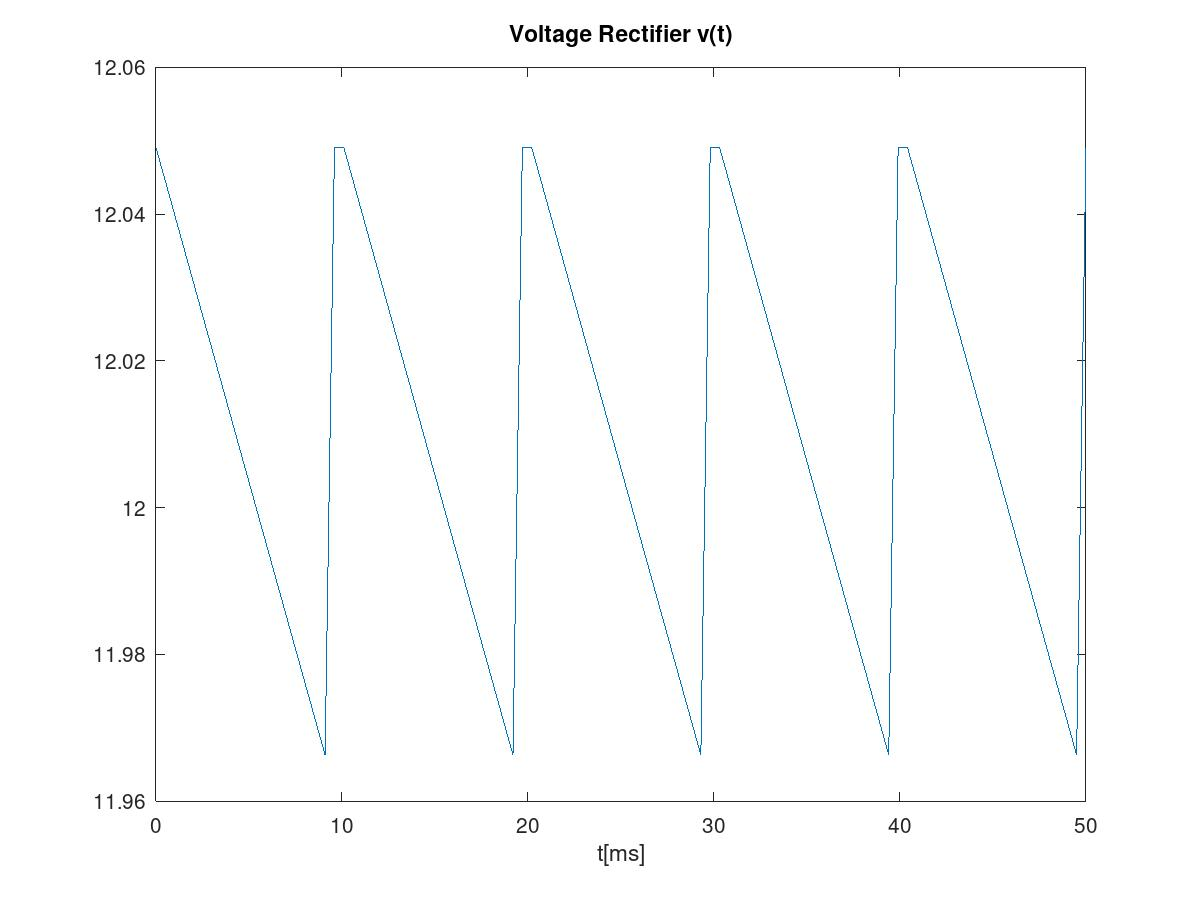
\includegraphics[width=0.75\linewidth]{../mat/voltage_rectifier.jpg}
    \caption{Evolution of the voltage at the ends of the 26 diodes during 5 semi-periods}
    \label{fig:Voltage Rectifier}
\end{figure}

\subsection{Voltage Ripple}
\label{subsec:2}

The voltage ripple is a consequence of the difficulty in converting a sinusoidal wave signal in a constant one. A 
bigger capacitance value in the capacitor $C_i$ lowers the current flow over time and so, it flattens the capacitor curve,
 allowing a smaller value for the ripple. \\
For a small ripple due to a good envelope regulator, $t_{off}$ can be approximated to the begining of the oscilation period and 
$t_{on}$ can be aproximated to half a period, and so, the voltage ripple can be approximatly calculated by $V_r = V_s (1-e^{\frac{-T}{2RC}})$.
Therefore, a bigger time constant allows a smaller ripple.

%\vspace{-4mm}
\begin{figure}[h] 
    \centering
    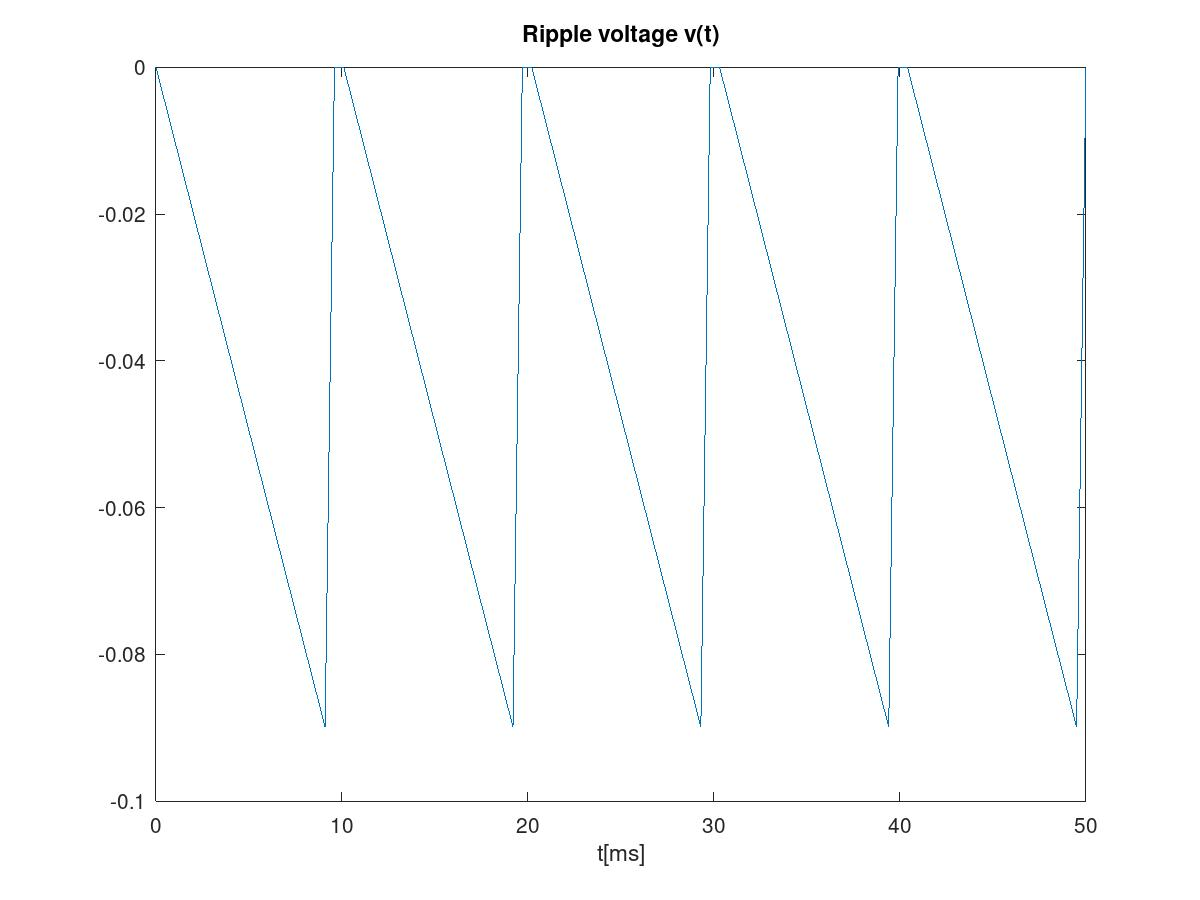
\includegraphics[width=0.75\linewidth]{../mat/vripple.jpg}
    \caption{Oscilations in the final voltage - ripple}
    \label{fig:Ripple}
\end{figure}

\vspace{4mm}
\begin{table}[ht]
    \centering
    \begin{tabular}{|c|c|}
        \hline
      {\bf Quantaties} & {\bf Volts} \\ \hline 
average & 1.200972e+01 \\ \hline 
ripple & 8.990121e-02 \\ \hline 
 deviation & 9.718317e-03 \\ \hline 

    \end{tabular}
    \vspace{10mm}
    \caption{Value of DC Output (V). Ripple Value (V).}
    \label{tab:teovalues}
  \end{table}

\newpage
